%\begin{figure*}[!t]
%    \centering
%    \begin{minipage}{0.5\textwidth}
%        \centering
%        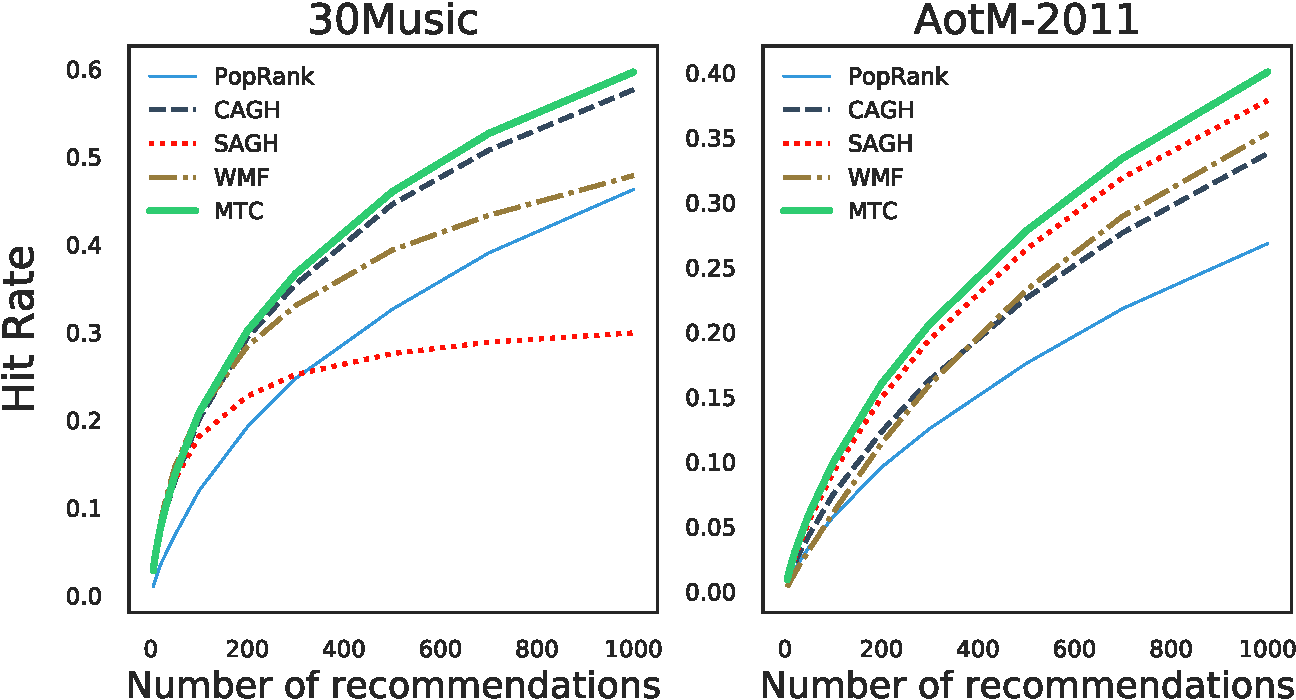
\includegraphics[width=.95\linewidth]{fig/hr3.pdf}
%        \caption{Hit rate of recommendation in the \emph{cold playlists} setting, \emph{higher} values indicate better performance.}
%        \label{fig:hr3}
%    \end{minipage}%\hspace{8pt}%
%    \begin{minipage}{.5\textwidth}
%        \centering
%        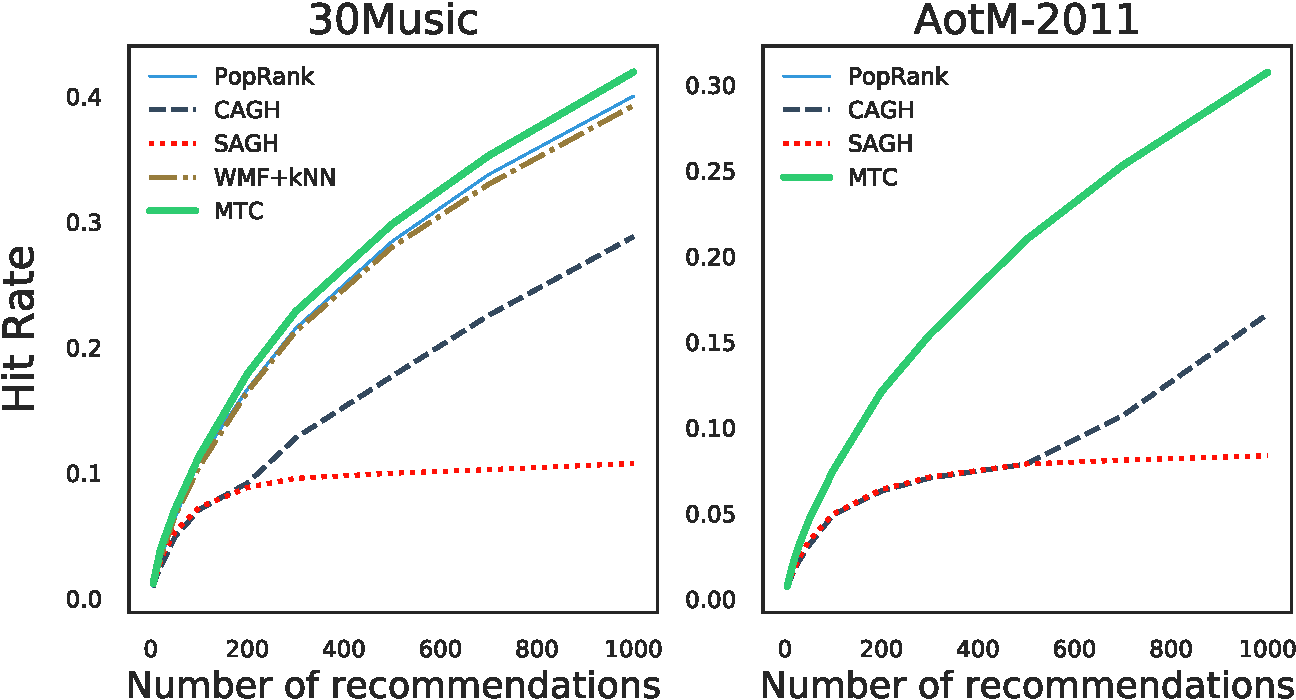
\includegraphics[width=.95\linewidth]{fig/hr4.pdf}
%        \caption{Hit rate of recommendation in the \emph{cold users} setting, \emph{higher} values indicate better performance.}
%        \label{fig:hr4}
%    \end{minipage}%\hspace{11pt}%
%    \begin{minipage}{0.5\textwidth}
%        \centering
%        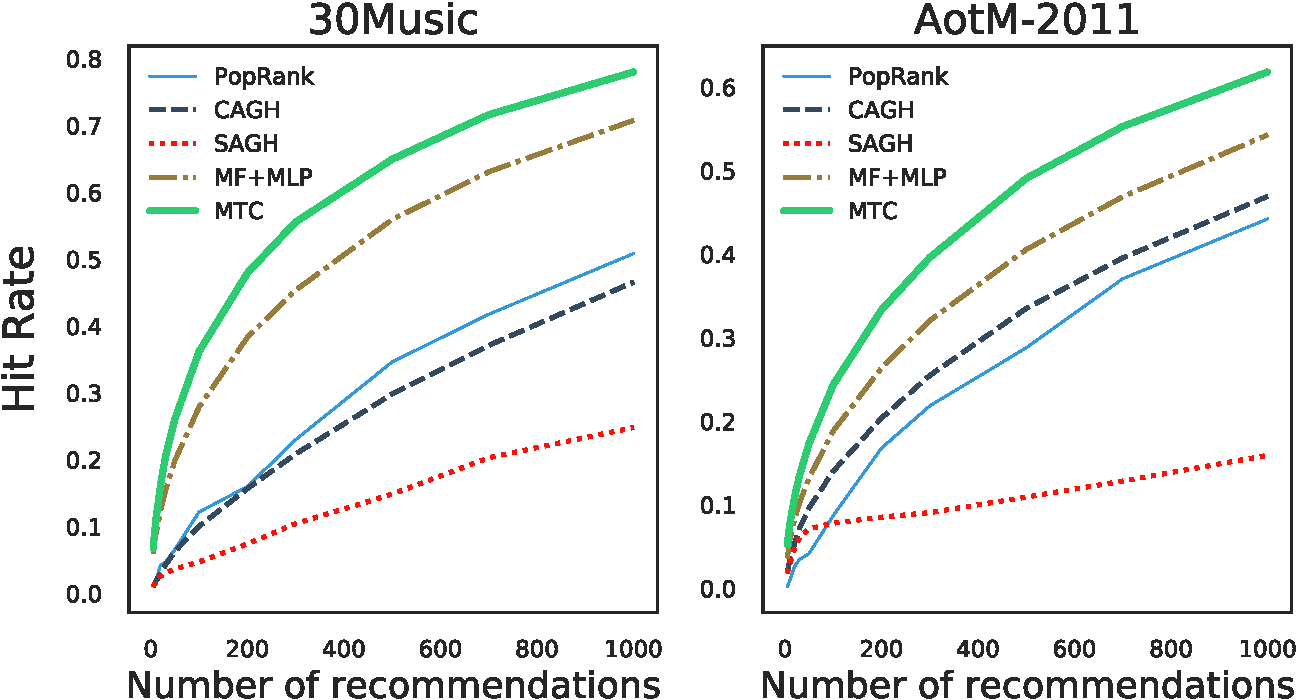
\includegraphics[width=.95\linewidth]{fig/hr1.pdf}
%        \caption{Hit rates for {\it cold songs}}
%        \label{fig:hr1}
%    \end{minipage}
%\end{figure*}

\begin{figure*}[!h]
    %\centering
    \begin{subfigure}[t]{.46\textwidth}
        \centering
        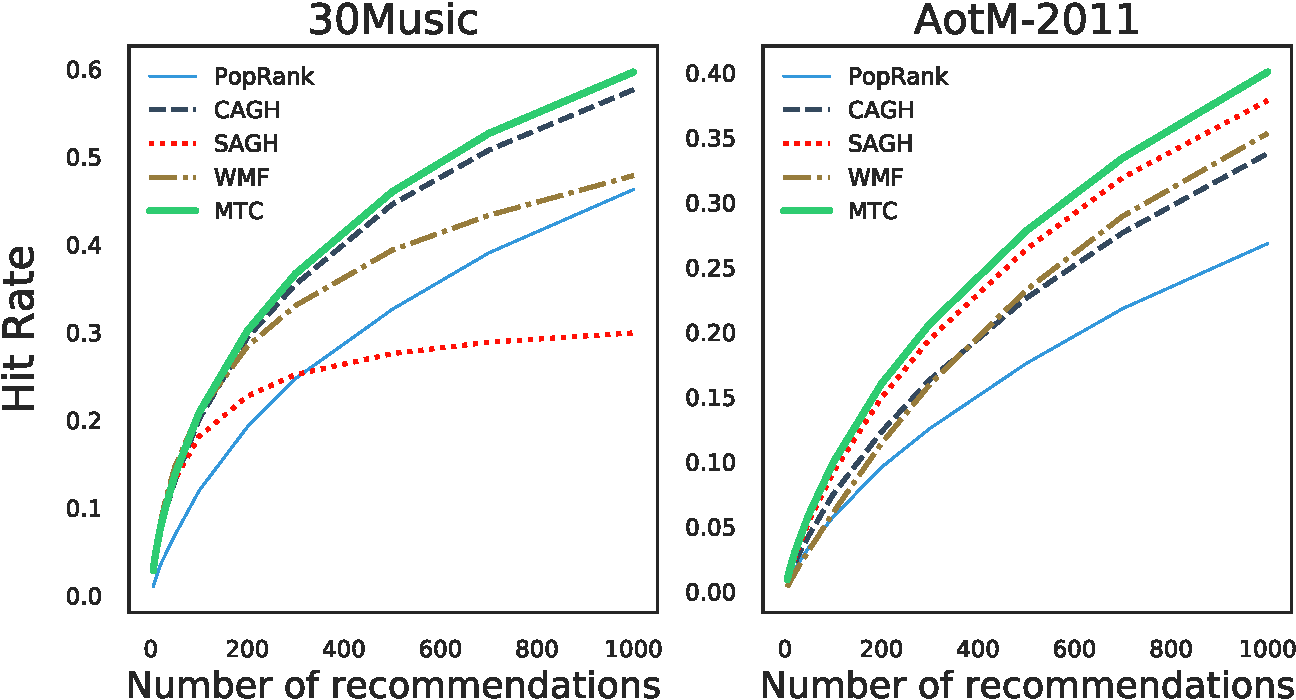
\includegraphics[width=\textwidth]{fig/hr3.pdf}
        \caption{Cold Playlists}
        \label{fig:hr3}
    \end{subfigure}\hspace{15pt}
    \begin{subfigure}[t]{.46\textwidth}
        \centering
        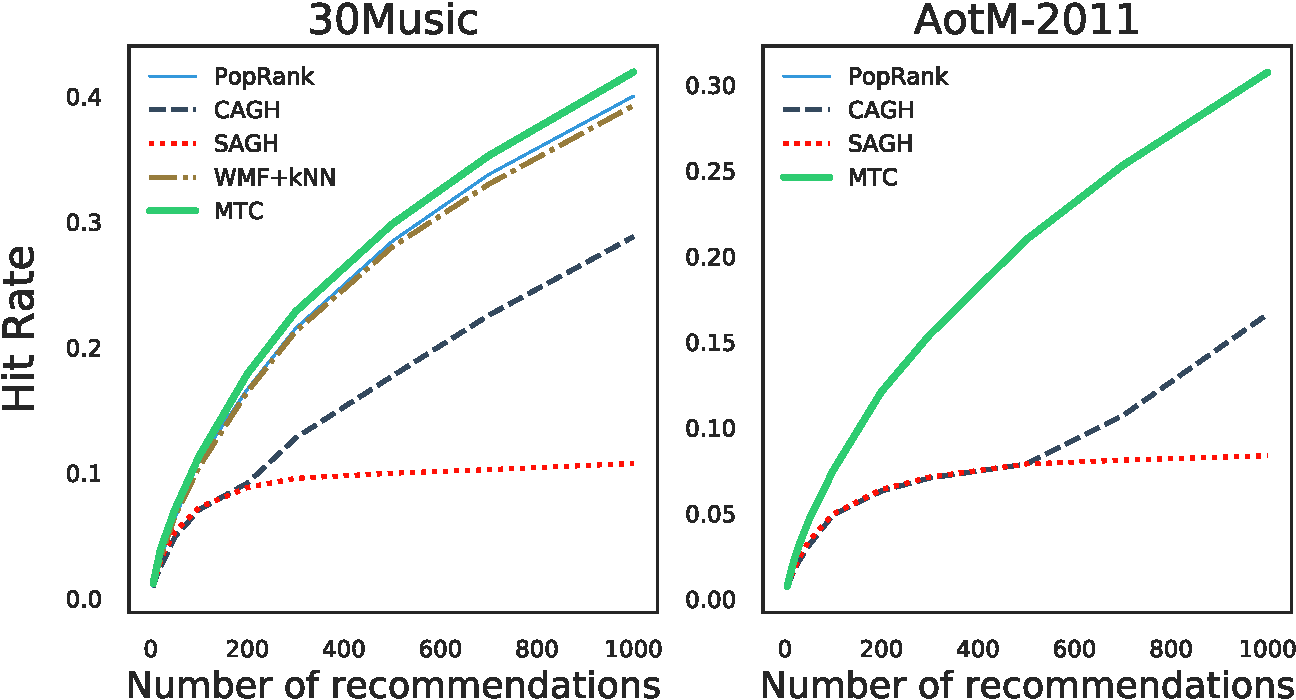
\includegraphics[width=\textwidth]{fig/hr4.pdf}
        \caption{Cold Users}
        \label{fig:hr4}
    \end{subfigure}
    \caption{Hit rate of recommendation in (a) \emph{cold playlists} setting, (b) \emph{cold users} setting, 
\emph{higher} values indicate better performance.}
\end{figure*}
